\documentclass[authordate, meta, issue]{jote-new-article}

\jissue{1}
\jvolume{4}
\jpages{20--21}
\paperissued{April 30, 2024}

\articletype{Special Issue - Meta Research}
\specialissue{Reflections on the Unintended Consequences of the Science Reform Movement}

\setcounter{page}{20}

\addbibresource{bibliography.bib}

\jotetitle{Reflections on Preregistration: Core Criteria, Badges, Complementary Workflows}
\keywordsabstract{badges, blind data analysis, Open Science, prospective registration, preregistration}
\abstracttext{Clinical trials are routinely preregistered. In psychology and the social sciences, however, only a small percentage of studies are preregistered, and those preregistrations often contain ambiguities. As advocates strive for broader uptake and effective use of preregistration, they can benefit from drawing on the experience of preregistration in clinical trials and adapting some of those successes to the psychology and social sciences context. We recommend that individuals and organizations who promote preregistration: (1) Establish core preregistration criteria required to consider a preregistration complete; (2) Award preregistered badges only to articles that meet the badge criteria; and (3) Leverage complementary workflows that provide a similar function as preregistration.}
\runningauthor{Thibault et al.}
\jname{Journal of Trial \& Error}
\acknowledgments{We thank Gustav Nilsonne, Steven Goodman, Mario Malički, Marton Kovacs, and Lisa Spitzer for feedback on earlier drafts of this commentary.}
\funding{Robert T. Thibault is supported by a general support grant awarded to METRICS from Arnold Ventures and a postdoctoral fellowship from the Canadian Institutes of Health Research. Marcus Munafo and Robert Thibault are part of the MRC Integrative Epidemiology Unit (MC\_UU\_00011/7). The funders have no role in the preparation of this manuscript or the decision to publish.}
\paperdoi{10.36850/mr6}
\paperreceived{November 17, 2022}
\author[1,2,3]{Robert T. Thibault\orcid{0000-0002-6561-3962}}
\affil[1]{Meta-Research Innovation Center at Stanford (METRICS), Stanford University.}
\affil[2]{School of Psychological Science, University of Bristol.}
\corremail{\href{mailto:robert.thibault@stanford.edu}{robert.thibault@stanford.edu}}
\corraddress{Stanford University}
\runningauthor{Thibault, Pennington, \& Munafò}
\author[4]{Charlotte R. Pennington\orcid{0000-0002-5259-642X}}
\affil[3]{MRC Integrative Epidemiology Unit at the University of Bristol.}
\author[2,3]{\mbox{Marcus R. Munafò\orcid{0000-0002-4049-993X}}}
\affil[4]{School of Psychology, Aston University.}
\paperaccepted{April 12, 2023}
\paperpublished{May 15, 2023}
\paperpublisheddate{2023-05-15}
\jwebsite{https://journal.trialanderror.org}
\jyear{2023}

\begin{filecontents}{bibliography.bib}
	@article{Abrams2020,
    title       = {Research Registries: {F}acts, Myths, and Possible Improvements},
    author      = {Abrams, E. and Libgober, J. and List, J.},
    volume      = {00703},
    url         = {https://ideas.repec.org//p/feb/artefa/00703.html},
    date        = {2020},
    journal     = {Artefactual Field Experiments, Article}
}


@article{Al-Durra2020,
    title       = {Prospective registration and reporting of trial number in randomised clinical trials: {G}lobal cross sectional study of the adoption of {ICMJE} and Declaration of Helsinki recommendations},
    author      = {Al-Durra, M. and Nolan, R. P. and Seto, E. and Cafazzo, J. A.},
    volume      = {369},
    url         = {https://doi.org/10.1136/bmj.m982},
    doi         = {10.1136/bmj.m982},
    date        = {2020},
    pages       = {982},
    journal     = {BMJ}
}


@article{Appelbaum2018,
    title       = {Journal article reporting standards for quantitative research in psychology: {T}he {APA}},
    author      = {Appelbaum, M. and Cooper, H. and Kline, R. B. and Mayo-Wilson, E. and Nezu, A. M. and Rao, S. M.},
    number      = {1},
    volume      = {73},
    url         = {https://doi.org/10.1037/amp0000191},
    doi         = {10.1037/amp0000191},
    date        = {2018},
    pages       = {3–25},
    journal     = {Publications and Communications Board task force report. The American Psychologist}
}


@article{Arnold2013,
    title       = {Double-Blind 2-Site Randomized Clinical Trial of Neurofeedback for {ADHD}},
    author      = {Arnold, L. E. and DeBeus, R.},
    url         = {www.clinicaltrials.gov.},
    date        = {2013},
    pages       = {02251743}
}


@article{Bakker2020,
    title       = {Ensuring the quality and specificity of preregistrations},
    author      = {Bakker, M. and Veldkamp, C. L. S. and van Assen, M. A. L. M. and Crompvoets, E. A. V. and Ong, H. H. and Nosek, B. A. and Soderberg, C. K. and Mellor, D. and Wicherts, J. M.},
    number      = {12},
    volume      = {18},
    url         = {https://doi.org/10.1371/journal.pbio.3000937},
    doi         = {10.1371/journal.pbio.3000937},
    date        = {2020},
    pages       = {3000937},
    journal     = {PLOS Biology}
}


@article{Berent2021,
    title       = {Candidate priming},
    author      = {Berent, M.},
    url         = {https://doi.org/10.17605/OSF.IO/F39KX},
    doi         = {10.17605/OSF.IO/F39KX},
    date        = {2021-08-23}
}

@online{BIHQUEST2023,
    date        = {2023},
    author      = {{BIH QUEST}},
    title       = {Charité Dashboard on Responsible Research},
    url         = {https://quest-dashboard.charite.de/#tabStart}
}


@article{Bosnjak2022,
    title       = {A template for preregistration of quantitative research in psychology: {R}eport of the joint psychological societies preregistration task force},
    author      = {Bosnjak, M. and Fiebach, C. J. and Mellor, D. and Mueller, S. and O’Connor, D. B. and Oswald, F. L. and Sokol, R. I.},
    number      = {4},
    volume      = {77},
    url         = {https://doi.org/10.1037/amp0000879},
    doi         = {10.1037/amp0000879},
    date        = {2022},
    pages       = {602},
    journal     = {American Psychologist}
}


@report{Campbell2019,
    author      = {Campbell, L. and Harris, K. and Flake, J. K. and Fried, E. I. and Beck, E. D. and Struhl, M. K. and Etz, A. and Lindsay, D. S. and Feldman, G. and van 't Veer, A. and Vazire, S.},
    url         = {https://osf.io/xv5rp/},
    date        = {2019}
}


@article{Chambers2022,
    title       = {The past, present and future of Registered Reports},
    author      = {Chambers, C. D. and Tzavella, L.},
    number      = {1},
    volume      = {6},
    url         = {https://doi.org/10.1038/s41562-021-01193-7},
    doi         = {10.1038/s41562-021-01193-7},
    date        = {2022},
    pages       = {29–42},
    journal     = {Nature Human Behaviour}
}


@article{Claesen2021,
    title       = {Comparing dream to reality: {A}n assessment of adherence of the first generation of preregistered studies},
    author      = {Claesen, A. and Gomes, S. and Tuerlinckx, F. and Vanpaemel, W.},
    number      = {10},
    volume      = {8},
    url         = {https://doi.org/10.1098/rsos.211037},
    doi         = {10.1098/rsos.211037},
    date        = {2021},
    pages       = {211037},
    journal     = {Royal Society Open Science}
}


@article{COS2016,
    title       = {Badges to Acknowledge Open Practices},
    author      = {{COS}},
    url         = {https://web.archive.org/web/20230420043737/https://osf.io/tvyxz/wiki/2.%20Awarding%20Badges},
    date        = {2016},
    journal     = {OSF}
}


@article{COS2023,
    title       = {Badges to Acknowledge Open Practices},
    author      = {{COS}},
    url         = {https://web.archive.org/web/20230508205525/http://web.archive.org/screenshot/https://osf.io/tvyxz/wiki/1.%20View%20the%20Badges/},
    date        = {2023},
    journal     = {OSF}
}


@article{DeAngelis2004,
    title       = {Clinical Trial Registration: {A} Statement from the},
    author      = {De Angelis, C. and Drazen, J. M. and Frizelle, F. A. and Haug, C. and Hoey, J. and Horton, R. and Kotzin, S. and Laine, C. and Marusic, A. and Overbeke, A. J. P. M. and Schroeder, T. V. and Sox, H. C. and Weyden, M. B. V. D.},
    number      = {12},
    volume      = {351},
    url         = {https://doi.org/10.1056/NEJMe048225},
    doi         = {10.1056/NEJMe048225},
    date        = {2004},
    pages       = {1250–1251},
    journal     = {International Committee of Medical Journal Editors. New England Journal of Medicine}
}


@article{DeVito2019,
    title       = {{FDAAA} TrialsTracker: {A} live informatics tool to monitor compliance with {FDA} requirements to report clinical trial results},
    author      = {DeVito, N. J. and Bacon, S. and Goldacre, B.},
    volume      = {266452},
    url         = {https://doi.org/10.1101/266452},
    doi         = {10.1101/266452},
    date        = {2019},
    journal     = {BioRxiv}
}


@thesis{DeVito2022,
    title       = {Trial registries for transparency and accountability in clinical research},
    author      = {DeVito, N. J.},
    publisher   = {University of Oxford},
    date        = {2022},
    type        = {Doctoral Thesis}
}


@article{Gabelica2022,
    title       = {Many researchers were not compliant with their published data sharing statement: mixed-methods study},
    author      = {Gabelica, M. and Bojčić, R. and Puljak, L.},
    date        = {2022},
    journal     = {Journal of Clinical Epidemiology}
}


@article{Hardwicke2021,
    title       = {Estimating the Prevalence of Transparency and Reproducibility-Related Research Practices in Psychology (2014–2017)},
    author      = {Hardwicke, T. E. and Thibault, R. T. and Kosie, J. E. and Wallach, J. D. and Kidwell, M. C. and Ioannidis, J. P. A.},
    volume      = {1745691620979806},
    url         = {https://doi.org/10.1177/1745691620979806},
    doi         = {10.1177/1745691620979806},
    date        = {2021},
    journal     = {Perspectives on Psychological Science}
}


@article{Hardwicke2023,
    title       = {Reducing bias, increasing transparency and calibrating confidence with preregistration},
    author      = {Hardwicke, T. E. and Wagenmakers, E. J.},
    volume      = {7},
    url         = {https://doi.org/10.1038/s41562-022-01497-2},
    doi         = {10.1038/s41562-022-01497-2},
    date        = {2023},
    pages       = {15–26},
    journal     = {Nat Hum Behav}
}


@article{Hardwicke2020,
    title       = {An empirical assessment of transparency and reproducibility-related research practices in the social sciences (2014–2017},
    author      = {Hardwicke, T. E. and Wallach, J. D. and Kidwell, M. C. and Bendixen, T. and Crüwell, S. and Ioannidis, J. P. A.},
    number      = {2},
    volume      = {7},
    url         = {https://doi.org/10.1098/rsos.190806},
    doi         = {10.1098/rsos.190806},
    date        = {2020},
    pages       = {190806},
    journal     = {Royal Society Open Science}
}


@article{Hopewell2022,
    title       = {An update to {SPIRIT} and {CONSORT} reporting guidelines to enhance transparency in randomized trials},
    author      = {Hopewell, S. and Boutron, I. and Chan, A.-W. and Collins, G. S. and de Beyer, J. A. and Hróbjartsson, A. and Nejstgaard, C. H. and Østengaard, L. and Schulz, K. F. and Tunn, R. and Moher, D.},
    url         = {https://doi.org/10.1038/s41591-022-01989-8},
    doi         = {10.1038/s41591-022-01989-8},
    date        = {2022},
    pages       = {1–4},
    journal     = {Nature Medicine}
}


@article{ICMJE2023,
    title       = {Recommendations for the Conduct, Reporting, Editing, and Publication of Scholarly Work in Medical Journals},
    author      = {{ICMJE}},
    url         = {https://web.archive.org/web/20230508211643/https://www.icmje.org/journals-following-the-icmje-recommendations/},
    date        = {2023}
}


@article{ICMJE2022,
    title       = {Journals stating that they follow the {ICMJE} Recommendations},
    author      = {{ICMJE}},
    url         = {https://web.archive.org/web/20230508211128/https://www.icmje.org/icmje-recommendations.pdf},
    date        = {2022}
}


@article{Lash2022,
    title       = {Getting Over {TOP}: {E}pidemiology},
    author      = {Lash, T. L.},
    url         = {https://journals.lww.com/epidem/fulltext/2022/01000/getting_over_top.1.aspx},
    date        = {2022}
}


@article{Lash2012,
    title       = {Should Preregistration of Epidemiologic Study Protocols Become Compulsory? {R}eflections and a Counterproposal},
    author      = {Lash, T. L. and Vandenbroucke, J. P.},
    number      = {2},
    volume      = {23},
    url         = {https://doi.org/10.1097/EDE.0b013e318245c05b},
    doi         = {10.1097/EDE.0b013e318245c05b},
    date        = {2012},
    pages       = {184–188},
    journal     = {EPIDEMIOLOGY}
}


@article{McPhetres2020,
    title       = {What should a preregistration contain?},
    author      = {McPhetres, J.},
    url         = {https://doi.org/10.31234/osf.io/cj5mh},
    doi         = {10.31234/osf.io/cj5mh},
    date        = {2020},
    journal     = {PsyArXiv}
}


@article{NC3Rs2021,
    title       = {{NC3R}s Funding Schemes Applicant and Grant Holder Handbook},
    author      = {{NC3Rs}},
    url         = {https://www.nc3rs.org.uk/sites/default/files/documents/Funding/Handbook.pdf},
    date        = {2021}
}


@article{Authority2021,
    title       = {Make it Public: {T}ransparency and openness in health and social care research},
    author      = {{NHS Health Research Authority}},
    url         = {https://www.hra.nhs.uk/planning-and-improving-research/policies-standards-legislation/research-transparency/make-it-public-transparency-and-openness-health-and-social-care-research/},
    date        = {2021}
}


@article{Nosek2018,
    title       = {The preregistration revolution},
    author      = {Nosek, B. A. and Ebersole, C. R. and DeHaven, A. C. and Mellor, D. T.},
    number      = {11},
    volume      = {115},
    url         = {https://doi.org/10.1073/pnas.1708274114},
    doi         = {10.1073/pnas.1708274114},
    date        = {2018},
    pages       = {2600–2606},
    journal     = {Proceedings of the National Academy of Sciences}
}


@article{Nosek2018b,
    title       = {Preregistration becoming the norm in psychological science},
    author      = {Nosek, B. A. and Lindsay, D. S.},
    volume      = {31},
    date        = {2018},
    journal     = {APS Observer}
}


@article{Sarafoglou2022,
    title       = {Comparing Analysis Blinding With Preregistration In The Many-Analysts Religion Project},
    author      = {Sarafoglou, A. and Hoogeveen, S. and Wagenmakers, E.-J.},
    url         = {https://doi.org/10.31234/osf.io/6dn8f},
    doi         = {10.31234/osf.io/6dn8f},
    date        = {2022},
    journal     = {PsyArXiv}
}


@article{Sarafoglou2022b,
    title       = {A survey on how preregistration affects the research workflow: {B}etter science but more work},
    author      = {Sarafoglou, A. and Kovacs, M. and Bakos, B. and Wagenmakers, E.-J. and Aczel, B.},
    number      = {7},
    volume      = {9},
    url         = {https://doi.org/10.1098/rsos.211997},
    doi         = {10.1098/rsos.211997},
    date        = {2022},
    pages       = {211997},
    journal     = {Royal Society Open Science}
}


@article{Scoggins2023,
    title       = {Measuring Transparency in the Social Sciences},
    author      = {Scoggins, B. and Robertson, M. P.},
    volume      = {14},
    date        = {2023},
    journal     = {Political Science and International Relations}
}


@article{Serghiou2021,
    title       = {Assessment of transparency indicators across the biomedical literature: {H}ow open is open?},
    author      = {Serghiou, S. and Contopoulos-Ioannidis, D. G. and Boyack, K. W. and Riedel, N. and Wallach, J. D. and Ioannidis, J. P. A.},
    number      = {3},
    volume      = {19},
    url         = {https://doi.org/10.1371/journal.pbio.3001107},
    doi         = {10.1371/journal.pbio.3001107},
    date        = {2021},
    pages       = {3001107},
    journal     = {PLOS Biology}
}


@article{Spitzer2021,
    title       = {Preregistration: {T}esting the Usability of the Psychological Research Preregistration-Quantitative ({PRP}-{QUANT}) Template},
    author      = {Spitzer, L. and Mueller, S. and Bosnjak, M.},
    date        = {2021}
}


@article{Srivastava2018,
    title       = {Sound Inference in Complicated Research: {A} Multi-Strategy Approach},
    author      = {Srivastava, S.},
    url         = {https://doi.org/10.31234/osf.io/bwr48},
    doi         = {10.31234/osf.io/bwr48},
    date        = {2018},
    journal     = {PsyArXiv}
}


@article{TARG2021,
    title       = {Estimating the prevalence of discrepancies between study registrations and publications: {A} systematic review and meta-analyses},
    author      = {{TARG Meta-Research Group} and {Collaborators}},
    url         = {https://doi.org/10.1101/2021.07.07.21259868},
    doi         = {10.1101/2021.07.07.21259868},
    date        = {2021}
}


@article{TARG2022,
    title       = {Discrepancy review: {A} feasibility study of a novel peer review intervention to reduce undisclosed discrepancies between registrations and publications},
    author      = {{TARG Meta-Research Group} and {Collaborators}},
    url         = {https://doi.org/10.1101/2022.01.18.22269507},
    doi         = {10.1101/2022.01.18.22269507},
    date        = {2022}
}


@article{Thabane2016,
    title       = {Methods and processes for development of a {CONSORT} extension for reporting pilot randomized controlled trials},
    author      = {Thabane, L. and Hopewell, S. and Lancaster, G. A. and Bond, C. M. and Coleman, C. L. and Campbell, M. J. and Eldridge, S. M.},
    number      = {1},
    volume      = {2},
    url         = {https://doi.org/10.1186/s40814-016-0065-z},
    doi         = {10.1186/s40814-016-0065-z},
    date        = {2016},
    pages       = {25},
    journal     = {Pilot and Feasibility Studies}
}

@article{Thibault2023,
        doi = {10.31222/osf.io/md2xz},
        url = {https://doi.org/10.31222/osf.io/md2xz},
        year = 2023,
        month = {may},
        publisher = {Center for Open Science},
        author = {Robert T. Thibault and Marton Kovacs and Tom Elis Hardwicke and Alexandra Sarafoglou and John P.A. Ioannidis and Marcus Robert Munafo},
        title = {Reducing bias in secondary data analysis via an Explore and Confirm Analysis Workflow ({ECAW}): A proposal and survey of observational researchers}
}

@article{vandenAkker2022,
    title       = {Selective Hypothesis Reporting in Psychology: {C}omparing Preregistrations and Corresponding Publications},
    author      = {van den Akker, O. and van Assen, M. A. L. M. and Enting, M. and de Jonge, M. and Ong, H. H. and Rüffer, F. and Schoenmakers, M. and Stoevenbelt, A. H. and Wicherts, J. and Bakker, M.},
    url         = {https://doi.org/10.31222/osf.io/nf6mq},
    doi         = {10.31222/osf.io/nf6mq},
    date        = {2022},
    journal     = {MetaArXiv}
}


@inbook{Weaver2022,
    title       = {Durchgeführt wie geplant?},
    author      = {Weaver, E. J. and Rehbein, S. T.},
    url         = {https://psycharchives.org/en/item/2462b05e-5d58-426b-8b43-a26556294a32},
    date        = {2022},
    booktitle     = {Ein detaillierter Vergleich zwischen Studien und ihren prä-registrierten Plänen}
}


@article{Organization2017,
    title       = {{WHO} Trial Registration Data Set (Version 1.3.1},
    author      = {{World Health Organization}},
    url         = {https://www.who.int/clinical-trials-registry-platform/network/who-data-set},
    date        = {2017}
}


@article{Zhang2020,
    title       = {{WHO} Trial Registration Data Set ({TRDS}) extension for traditional Chinese medicine 2020: {R}ecommendations, explanation, and elaboration},
    author      = {Zhang, X. and Lan, L. and Chan, J. C. P. and Zhong, L. L. D. and Cheng, C.-W. and Lam, W.-C. and Tian, R. and Zhao, C. and Wu, T.-X. and Shang, H.-C. and Lyu, A.-P. and Bian, Z.-X.},
    number      = {1},
    volume      = {20},
    url         = {https://doi.org/10.1186/s12874-020-01077-w},
    doi         = {10.1186/s12874-020-01077-w},
    date        = {2020},
    pages       = {192},
    journal     = {BMC Medical Research Methodology}
}
\end{filecontents}

\begin{document}



\begin{frontmatter}
  \maketitle
  \begin{abstract}
    \printabstracttext
  \end{abstract}
\end{frontmatter}






\lettrine{C}{linical} trials are routinely preregistered\footnote{ Clinical trials research uses the term \emph{prospective registration, }whereas other disciplines (including psychology and the social sciences) use the term \emph{preregistration. }Prospective registration of clinical trials differs from preregistration of research in other disciplines in terms of its history, the functions it was designed to serve, and implementation details (e.g., clinical trial registries do not include sections specifically dedicated to hypotheses or analysis plans) \parencites[explanation adapted from: ][]{TARG2022}. To streamline the reading of this commentary, we use the term \emph{preregistration} for both clinical trials and other disciplines.} \parencites{Al-Durra2020}. However, in other fields such as psychology and the social sciences only a small percentage of studies are preregistered,\footnote{ Randomly sampled publications from the years 2014-2017 found that 1-5\% (95\% confidence intervals) of studies in psychology and 0-1\% (95\% CI) of studies in the social sciences were preregistered \parencites{Hardwicke2020}{Hardwicke2021}. Another study found that 5\% of over 90,000 articles in political science and international relations published from 2010-2021 were preregistered, but that 16\% were preregistered in 2021 \parencites{Scoggins2023}. Other sources also indicate an increase in the prevalence of preregistration since Hardwicke et al.’s 2014-2017 sample. For example, there were ~12,000 OSF preregistrations from 2012-2017 \parencites{Nosek2018b}, but \href{https://web.archive.org/web/20230126224417/https\%3A\%2F\%2Fosf.io\%2Fregistries\%2Fdiscover}{over 100,000 across a similar time period from 2018 to January 2023}. Some of these preregistrations, however, may be duplicates (e.g., to update a preregistration, \href{https://web.archive.org/web/20230131232333/https\%3A\%2F\%2Fhelp.osf.io\%2Farticle\%2F156-update-your-registration}{the OSF instructs users to create a new preregistration}). The prevalence of preregistration in psychology and the social sciences likely remains far below that of clinical trials research.} and they often contain ambiguities in the description of their study design, hypotheses, and analysis plans \parencites{Bakker2020}{vandenAkker2022}. As advocates strive for broader uptake and more effective use of preregistration, the research community could benefit from drawing on the success of preregistration in clinical trials, where preregistration is commonplace.\footnote{ For example, 92\% of UK clinical trials submitting a final report to the NHS Health Research Authority in Sep 2021 to Sep 2022 are registered in a publicly accessible database \parencites{Authority2021}; 75\% of German clinical trials that were registered in 2017 were done so prospectively \parencites{BIHQUEST2023}, and 71\% of clinical trials published in PubMed-indexed journals in 2018 were registered, although only 42\% were registered before the study began (i.e., \underline{pre}registered) \parencites{Al-Durra2020}.} Preregistered clinical trials contain itemized and relatively explicit outcome measures, and most report their results.\footnote{ As of March 2023, for clinical trials that were completed over 12 months ago, \href{https://fdaaa.trialstracker.net/}{76\% of those covered under the Food and Drug Administration Amendments Act }and \href{https://eu.trialstracker.net/}{84\% of those posted on the European Union Clinical Trials Register (EUCTR)} contained a link in their preregistration pointing to the reported results. Notably, however, reported outcomes do not always match preregistered outcomes (see footnote 7).}







We propose three actions for the research community to consider to improve the function of preregistration in psychology and the social sciences (see Table 1 \& Box 1). These proposals stem from insights developed while conducting research on preregistration across disciplines, including meta-analyses of discrepancies between preregistrations and published manuscripts \parencites{TARG2021} and a feasibility study of a peer review intervention to address these discrepancies before publication \parencites{TARG2022}. We discuss the function of preregistration in terms of reducing bias and making risk of bias transparent \parencites[as outlined in][]{Hardwicke2023}, as well as the auxiliary benefit of improved research quality.\footnote{ We acknowledge that there are ongoing debates about the function, purpose, and goals of preregistration \parencites[e.g.,][]{McPhetres2020}. We feel that this debate does not preclude implementation of our suggestions.} Our proposals are by no means exhaustive; more comprehensive overviews of preregistration are available elsewhere \parencites[e.g.,][]{Hardwicke2023}{DeVito2022}.







We propose that advocates for preregistration consider to:

\begin{fullwidth}
  \begin{enumerate}[leftmargin=!,itemindent=0pt]

    \item \textbf{Establish core preregistration criteria }(i.e., a minimum amount of information required to consider a preregistration complete—as the World Health Organization’s International Clinical Trials Registry Platform has done for clinical trial registration).


    \item \textbf{Award preregistered badges only to articles that meet the badge criteria }(of which few currently do).


    \item \textbf{Leverage complementary workflows that provide a similar function as preregistration }(e.g., blinded data analysis to minimize data-dependent analytical decisions).


  \end{enumerate}
\end{fullwidth}




\begin{table*}
  \begin{fullwidth}

    \caption[ashtash]{ \textbf{Problems and proposed solutions for preregistration in psychology and the social sciences. }}
    \begin{tabularx}{\textwidth}{@{} >{\arraybackslash\RaggedRight}X  >{\arraybackslash\RaggedRight}X @{}}
      \toprule
      \textbf{Problem} &
      \textbf{Proposed solutions}\textsuperscript{\textbf{*}}
      \\
      \midrule

      \begin{enumerate}
        \item Low uptake of preregistration
        \item Imprecise and ambiguous preregistrations
        \item Poor alignment between preregistrations and manuscripts
      \end{enumerate}
                       &

      {
          \renewcommand{\theenumi}{\Alph{enumi}}
          \begin{enumerate}

            \item  Establish core preregistration criteria
            \item      Award preregistered badges only to articles that meet the badge criteria
            \item Leverage complementary workflows that provide a similar function as preregistration
          \end{enumerate}}
      \\
      \bottomrule
    \end{tabularx}
    {\small \RaggedRight

    \begin{enumerate}
      \item Preregistration provides additional benefits once a substantial proportion of studies are preregistered—such as facilitating evidence synthesis and reducing duplication.
      \item Imprecise language and ambiguities in preregistrations leave them open to various interpretations, and in turn, limit their ability to reduce bias and transparently communicate study plans.
      \item Poor alignment between preregistrations and manuscripts—both in terms of the overall structure of the documents as well as the specific content—make it difficult to compare the texts to assess risk of bias.
    \end{enumerate}
    The solutions we propose are partial solutions in the sense that they remain unlikely to fully solve shortcomings in preregistration. They can be implemented individually or alongside other efforts.

    \textsuperscript{\textbf{*}}We itemize the \emph{problems} with numbers and the \emph{proposed solutions} with letters to indicate that they are not aligned in a one-to-one manner; each proposed solution could impact each of the three problems to different extents.}

    \label{tab:table1}
  \end{fullwidth}
\end{table*}


\section{1. Establish core preregistration criteria}


For clinical trials to be considered fully registered, they must provide information regarding 24 specific items, known as the Trial Registration Data Set \parencites{Organization2017}. Although these 24 items do not include a detailed analysis plan, they set a minimal standard that organizations such as the International Committee of Medical Journal Editors can promote \parencites{ICMJE2022}{ICMJE2023}. This itemized standard laid the foundation for regulations and institutional infrastructure, which in turn drove the widespread uptake of preregistration in clinical trials.\footnote{ For example, in 2005, the International Committee of Medical Journal Editors (ICMJE) made preregistration a necessary condition for consideration for publication \parencites{DeAngelis2004}. \href{http://web.archive.org/save/https://clinicaltrials.gov/ct2/resources/trends}{Clinical trial registration rates quadrupled in 2005} and thousands of journals now claim to follow this policy \parencites{ICMJE2023}.} It allows for transparent updating of preregistrations and makes comparisons between preregistrations and publications relatively easy (see Figure 1). The structure is sufficiently clear-cut, such that the Health Research Authority in the UK now uses information from ethics applications to register trials on behalf of clinical trialists \parencites{Authority2021}. These researchers can go beyond the minimum 24 items, add as many details as they would like to the registration, and append a study protocol.\footnote{ Notably, clinical trial preregistration is not a panacea. Some trials are never preregistered; among those that are, about one-third publish at least one different primary outcome than what was preregistered, and about two-thirds publish at least one different secondary outcome than what was preregistered \parencites{TARG2021}. While some researchers challenge the usefulness of clinical trial preregistration based on this situation \parencites[e.g.,][]{Lash2022}{Abrams2020}, it is trial preregistration that allows us to identify this risk of bias. Without preregistration, we would not be able to quantify the level of selective reporting or publication bias. Moreover, preregistering protocols—which include statistical analysis plans—remains rare in biomedicine broadly \parencites{Serghiou2021}.}







In contrast to clinical trial registrations which include discrete items followed by short responses (e.g., primary outcome; sample size), preregistration templates in psychology and the social sciences often include broad headers followed by blocks of text (e.g., hypotheses, analysis plan—see Figure 1).\footnote{ Granted, the scope of preregistration must be expanded to capture the breadth of study designs used in psychology and the social sciences, as compared to the more limited design options used in clinical trials.} Single hypotheses can contain multiple elements that would be better divided into several distinct hypotheses. Preregistrations sometimes list several variables and analyses but provide a sample size calculation for only one analysis. Within a preregistration, aligning a single hypothesis to its outcome measure and analysis can be far from trivial. Matching these to text in the manuscript presents an additional challenge. Thus, the less structured information provided in many psychology preregistrations can obscure a reader’s understanding of what the researchers planned to do and whether they did it.\footnote{ We have no qualms when researchers deviate from a preregistration, so long as they disclose the deviation when reporting results. In many cases, deviations are entirely justifiable and can be necessary to improve a study design or analysis.}\textsuperscript{,}\footnote{ One complication for preregistration in psychology and the social sciences, as compared to clinical trials, is that the spectrum of research questions ranges from highly exploratory to purely confirmatory. Some ambiguities in preregistrations may arise when researchers attempt to present exploratory research questions in a confirmatory format.}





\begin{figure*}[t]
  \begin{fullwidth}
    \label{fig:rId9}

    % 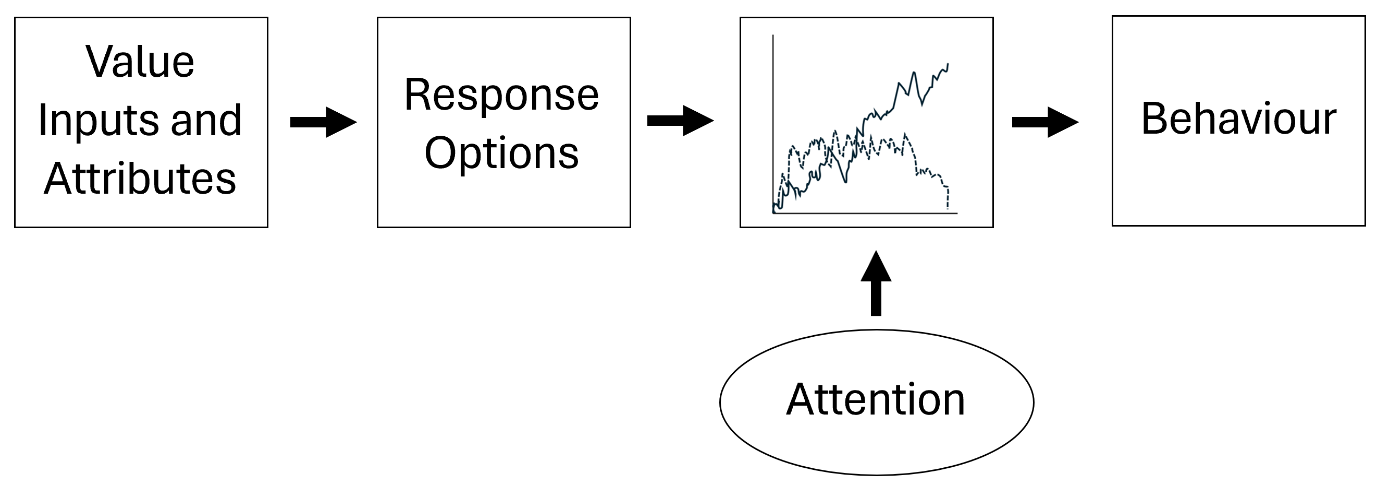
\includegraphics[height=.24\paperheight]{media/image2.png}
    % 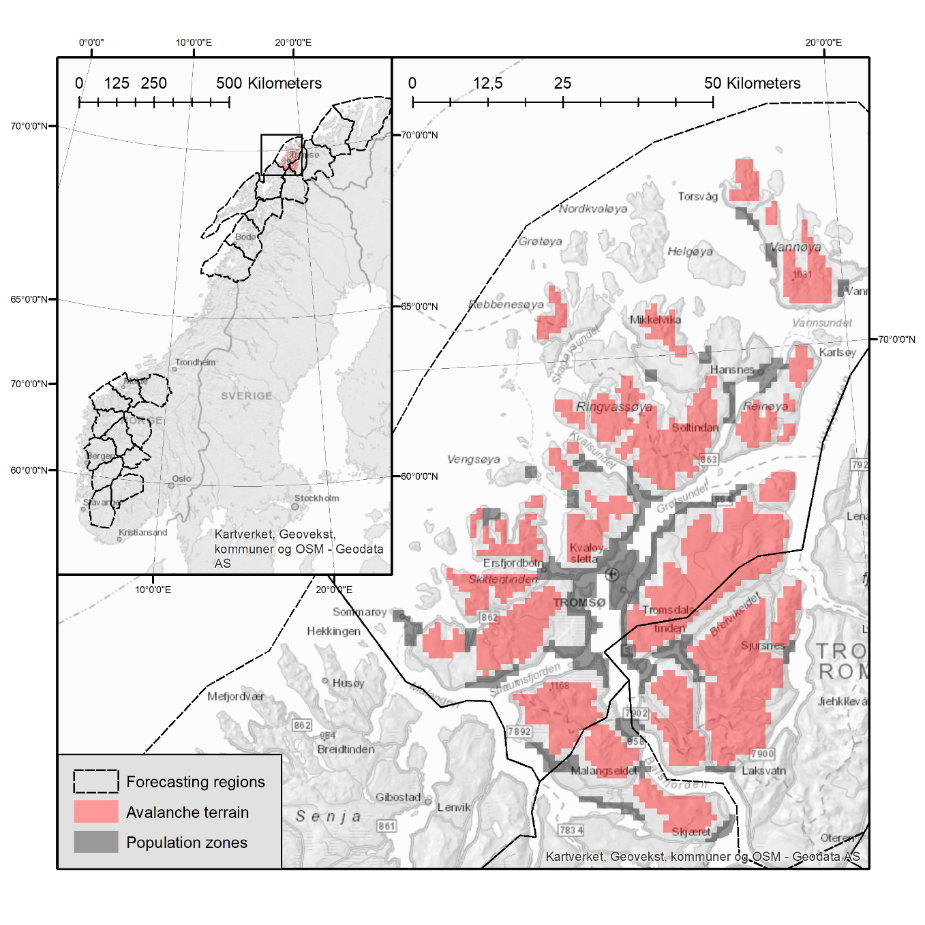
\includegraphics[width=.24\paperheight]{media/image3.png}
    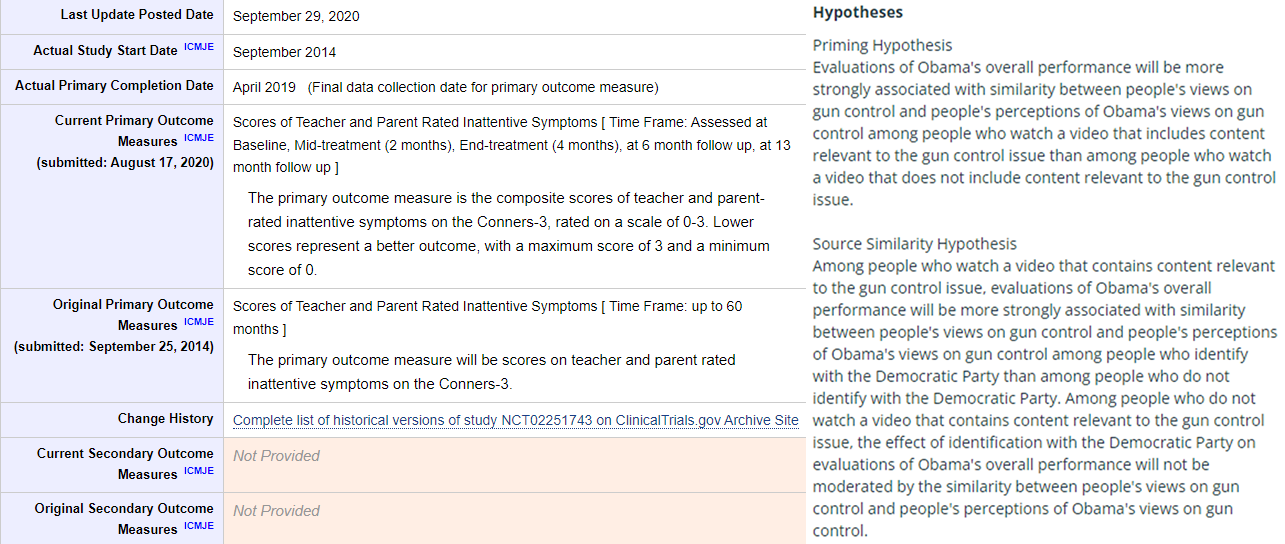
\includegraphics[width=\linewidth]{media/image4.png}

    \caption[check]{\textbf{Comparison of a clinical trial preregistration excerpt (left) to an OSF preregistration excerpt (right)}\protect\textsuperscript{*}. The clinical trial preregistration excerpt demonstrates several features that the psychology and social sciences community could benefit from considering. These include: (1) The option for an itemized and tabular format; (2) Clear demarcation of the 24 items contained in the WHO Trial Registration Data Set, which is supported by the International Committee of Medical Journal Editors and demarcated with the superscript \textsuperscript{ICMJE}; (3) Clear demarcation of the primary outcome measure and time frame of assessment; (4) Easy identification of updates to the primary outcome measure (e.g., several time points were added); (5) Easy identification of core items that are not provided (e.g., secondary outcome measures); and (6) A link to a \emph{Change History} log, which looks similar to a Microsoft Word document with track changes. The OSF has recently begun to provide a function allowing researchers to update their preregistration. The updated preregistration identifies sections that were updated (e.g., “Hypotheses”), but does not provide the track-changes style functionality that clinicaltrials.gov does. OSF preregistrations also often contain a statistical analysis plan whereas clinical trial preregistrations rarely do.\\  {\footnotesize\textsuperscript{*} \emph{These excerpts are copied from \parencites{Arnold2013} and \parencites{Berent2021}. We selected the clinical trials registration because the lead author (RTT) was familiar with it, and it clearly depicts several benefits of clinical trial preregistrations in a relatively small screenshot. The OSF registration was selected by going to \href{http://www.osf.io/registries}{www.osf.io/registries} and selecting \emph{Provider}: “OSF Registries” and \emph{OSF Registration Type}: “OSF Preregistration,” and then choosing a recent preregistration that depicts the text-block response format. }}}

  \end{fullwidth}
\end{figure*}









Given the low prevalence of preregistration in psychology and social sciences research \parencites{Hardwicke2020}{Hardwicke2021}{Scoggins2023}, alongside the difficulty of comparing preregistered study details to published study reports \parencites{TARG2022}{vandenAkker2022} we argue that establishing core preregistration criteria would complement ongoing initiatives that strive for ideal practice.\footnote{Some researchers propose that publications of preregistered studies should include a section outlining deviations from the preregistration \parencites[e.g.,][]{Campbell2019}. While we agree with these initiatives, sections on deviations will be difficult to interpret if preregistrations are highly ambiguous due to a lack of itemization. }







Efforts have been made to create standard preregistration templates in psychological science (e.g., Open Science Framework, AsPredicted), but these can vary substantially, and there is no broad agreement regarding the details they must include. In an attempt toward standardization, a Preregistration Task Force consisting of the American Psychological Association (APA), the British Psychological Society (BPS), and the German Psychological Society (DGP), supported by the Center for Open Science (COS) and the Leibniz Institute for Psychology, developed a consensus template\footnote{Although the authors use the terms \emph{consensus }and \emph{consensus template} throughout their manuscript, there is no description of the consensus process, which may not have been formalized.} for the preregistration of quantitative psychology research \parencites[the PRP-QUANT template;][]{Bosnjak2022}. On the one hand, the template is exhaustive and was purposefully designed to parallel the structure of the APA Style Journal Article Reporting Standards \parencites{Appelbaum2018}; its proper use would present a very effective implementation of preregistration. On the other hand, there is no evidence that user-testing informed the template\footnote{ Two of the authors are now testing the usability of the PRP-QUANT template \parencites[preregistration:][]{Spitzer2021}.} and its uptake remains limited at this time.\footnote{ This manuscript was first posted as a preprint in February 2021 and has received 27 citations (according to Google Scholar on 31 Jan 2023). These citations appear to mostly reference, rather than use, the PRP-QUANT template. If this template serves a broad user base, is user-friendly, and strongly supported by the organizations involved in making the template (some of the leading psychology organizations in the world), we would predict a greater uptake to date, though increased uptake may occur in the years to come. \href{https://www.psycharchives.org/en/browse/?q=zpid.tags.visible\%3APRP-QUANT}{As of April 2023, it appears the template has been used up to 75 times on the PsychArchives repository.} }







Comparable guidelines in clinical trials have been developed through formal consensus processes that involve diverse stakeholders, include a user-testing stage (i.e., piloting), and are widely used by researchers.\footnote{For example, the Consolidated Standards of Reporting Trials (CONSORT), the Standard Protocol Items: Recommendations for Interventional Trials (SPIRIT) \parencites{Hopewell2022}.} These documents were designed to apply across clinical trials research, regardless of the specific discipline. Their structure is such that researchers can create extensions to the guidelines to target their specific disciplines more fully \parencites[e.g., traditional Chinese medicine:][]{Zhang2020}[pilot trials:][]{Thabane2016}. Core preregistration criteria could be developed through a similar process and designed to accommodate the diversity of study types in psychology and the social sciences. They could facilitate broad adoption of preregistration by setting a minimum standard that is relatively easy to achieve and a benchmark upon which publishers, funders, and institutions can develop regulations.







\section{2. Award preregistered badges only to articles that meet the badge criteria}



As of April 2023, the Center for Open Science website lists 80 journals that award badges to articles that claim to have used open science practices such as preregistration, open materials, and open data (\url{www.cos.io/initiatives/badges}). To receive a preregistered badge, a publication should have no undisclosed discrepancies from the preregistration \parencites{COS2023}. And yet, two studies analyzing psychology publications with preregistered badges found that 89\% of 27 articles contained at least one undisclosed discrepancy \parencites{Claesen2021}\footnote{ Researchers replicated and extended this study and found comparable results \parencites{Weaver2022}.} and 67\% of 258 articles selectively reported at least one hypothesis \parencites{vandenAkker2022}.\footnote{ This sample also includes studies without a preregistered badge, although most articles did have a preregistered badge. They sampled from two populations: articles that contained a preregistered badge and articles that earned a Preregistration Challenge Prize from the Center for Open Science. Their manuscript, however, only reports summary results across both samples.} The organization that developed the badges—the Center for Open Science—describes two ways to award badges: author self-disclosure or peer review \parencites{COS2016}.







\subsection{Disclosure}

Some journals, in their instructions for authors, state that they use the self-disclosure method to award badges (e.g., \href{https://www.psychologicalscience.org/publications/psychological_science/ps-submissions}{\emph{Psychological Science}}, \href{https://www.elsevier.com/journals/journal-of-experimental-social-psychology/0022-1031/guide-for-authors}{\emph{Journal of Experimental Social Psychology}}), but the disclosure statement provided by the COS which these journals use does not align with the preregistered badge criteria. The four criteria for a preregistered badge are: “(1) A public date-time stamped registration is in an institutional registration system; (2) Registration pre-dates the intervention; (3) Registered design corresponds directly to reported design; and (4) Full disclosure of results in accordance with registered plan” \parencites{COS2023}. However, the disclosure form used by these journals asks authors to complete five disclosure items \parencites{COS2016}, none of which match the third and fourth badge criteria. Thus, authors can both truthfully complete the disclosure form and not meet the badge criteria. Even if the disclosure items were realigned to match the badge criteria, it remains unclear whether the proportion of badged papers that fully meet all criteria would rise in the absence of a verification mechanism.







\subsection{Peer review}

We are not aware of any journal that systematically peer reviews articles to ensure they meet the criteria for a preregistered badge. Moreover, based on our experience \parencites{TARG2022} and that of other researchers who have systematically examined publications awarded with a preregistered badge (Olmo van den Akker, personal communication, 2021; Aline Claesen, personal communication, 2019), we feel it is very difficult to confidently state that the “Registered design corresponds directly to reported design” or “Full disclosure of results in accordance with registered plan.” Indeed, one study found that researchers could only agree on the number of hypotheses present in 14\% of preregistrations \parencites{Bakker2020}. Another study with a strict operationalization of what constituted a hypothesis had 54\% agreement between coders regarding the number of hypotheses \parencites{vandenAkker2022}. The lack of itemized core preregistration criteria alongside differences in the structure of preregistrations and manuscripts renders many comparisons ambiguous.







One could argue that the issues we present regarding inaccurate awards are outweighed by the benefit that badges may have on the uptake of preregistration. Indeed, the badge criteria were designed to represent a high aspirational standard, rather than setting a minimal bar. However, there is a possibility that badges in their current implementation have negative effects. Given that most articles awarded a preregistered badge do not fully meet the criteria for earning that badge, awarding badges can create a false impression that rigorous research practices are being used and therefore lend undue trust to studies awarded a preregistered badge. This practice could also have downstream impacts on the trustworthiness of these types of initiatives more broadly.\footnote{ For example, as has happened for “data available upon request” statements, where over 90\% of requests go unanswered or are declined \parencites{Gabelica2022}.}







Changing the criteria for the preregistered badge could be one way to make clearer what the badge signals. They could be revised, for example, to require only the existence of a permanent and public preregistration in a repository that provides a DOI, without requiring that the preregistration was followed. This criterion would be easy to audit\footnote{ Auditing could be conducted by any one of various stakeholders—for example, by the journals who reward the badges, the organization who developed them (COS), funders, researchers \parencites[e.g., similar to the \href{http://web.archive.org/save/https://fdaaa.trialstracker.net/}{FDAAA Trials Tracker}][]{DeVito2019}, or institutions (e.g., similar to the \href{http://web.archive.org/save/https://quest-dashboard.charite.de/}{Charité Dashboard on Responsible Research}).} and achieves at least one main function that preregistration was designed to address—putting a timestamp on study plans to help demarcate confirmatory research \parencites{Nosek2018}. An additional criterion could demand that the preregistration include all the items in an established core preregistration criteria, as outlined earlier in this commentary. Machine-readable preregistration statements could also be employed to facilitate automated compliance monitoring from funders or institutions. Based on the current badge criteria, a publication whose preregistration has almost no detail could earn a preregistered badge, whereas a publication with a very detailed preregistration and a minor discrepancy should not earn a badge.\footnote{ Although in practice, badges appear to be awarded in both cases. When appropriately disclosed, we have no qualms with discrepancies.}







Taken together, current practices for awarding preregistered badges reward researchers even if their preregistration is of low quality and aligns poorly with the associated publication. We commend the development and testing of new initiatives; at the same time, we advocate for follow-up and evaluation to investigate whether they work as intended.







\section{3. Leverage complementary workflows that provide a similar function as preregistration }



Preregistration can reduce bias, increase transparency, and may also improve research quality \parencites{Hardwicke2023}{Sarafoglou2022b}. However, there are no checks and balances to evaluate whether the study outlined in a preregistration is well designed or clearly described \parencites[except when using the Registered Reports format; see][]{Chambers2022}. Journal policies and peer review can improve the quality of reporting in relation to a preregistration, but they occur too late in the research pipeline to impact the study design or preregistration quality. Complementary research workflows could achieve some of the same functions as preregistration and may come with additional benefits (e.g., blind data analysis, Experimental Design Assistants, protocol peer review).\footnote{See \textcite{Srivastava2018} for a more in-depth discussion of various alternatives and complementary strategies to typical preregistration.}







For observational research, data management organizations could employ workflows that necessitate open research practices. For example, they could provide researchers with a synthetic dataset, which researchers could use to develop an analysis script. The researchers would then run their analysis in a Trusted Research Environment (TRE) where the results are output, the real data remains hidden, and the analysis is logged and made public (e.g., as done at OpenSAFELY.org). If a Trusted Research Environment is not available, data management organizations could simply provide the complete dataset after the researchers register their analysis script \parencites[e.g., as done in][]{Sarafoglou2022}[and surveyed in][]{Thibault2023}. These workflows make executable analyses—as opposed to sometimes ambiguous blocks of text—publicly available, while also protecting researchers from making data-dependent analytical decisions. They also overcome arguments raised against preregistration for observational research, including that the data often already exist, knowledge of the data may be necessary to devise a reasonable analysis plan, and registration can inhibit exploration \parencites{Lash2012}.







Researchers can execute a comparable workflow for experimental studies by writing an analysis script based on simulated data and preregistering it before beginning data collection. In other words, the preregistration would include a results section based on a simulated dataset and the numbers are simply updated after running the analysis on the real data.







Another research tool—the Experimental Design Assistant—can be employed in a similar manner. This web application, developed by The National Centre for the Replacement, Refinement and Reduction of Animals in Research (NC3Rs), uses a graphical interface to walk preclinical animal researchers through designing their experiment. Unlike preregistration, the EDA is an interactive tool that prompts users to input thorough information and gives warnings when the input fails to align. It then outputs a PDF which the NC3Rs encourages researchers to append to funding applications sent to their organization \parencites{NC3Rs2021}. This tool holds the potential to simultaneously help researchers design effective experiments and reduce their workloads by using the PDF output as a component of a preregistration.




\begin{table}[b!]
  \begin{fullwidth}
    \begin{tabularx}{\textwidth}{@{} X @{}}
      \textbf{Box 1. Agents of change} \\
      Our three recommendations target the research community broadly and differ in their implementation pathways. Establishing core preregistration criteria would require coordination across various stakeholders including publishers, funders, institutions, learned societies, researchers, and other end-users of research findings. Such an initiative would take a concerted effort and could gain momentum through a grassroots push from researchers or a top-down mechanism from major funders. In contrast, any journal can improve their own use of preregistered badges, and the organization who created them—the Center for Open Science (COS)—holds the ability to redefine the badge criteria. As for our final recommendation, any individual research group, funder, data management organization, or other stakeholder can explore the use of complementary workflows. Highly successful workflows could then be adopted more widely.
    \end{tabularx}
  \end{fullwidth}
\end{table}






These examples hold the potential to increase the uptake of preregistration and improve the precision of preregistrations. They do so by embedding the research pipeline with a user-friendly workflow that documents precise study plans.








\section{Conclusion}



In psychology and the social sciences, preregistrations can reduce bias and improve transparency. At the same time, they remain underused, can lack clarity, and are often difficult to compare directly with their associated publication. Current efforts to promote the uptake of preregistration (e.g., badges) and improve preregistration quality (e.g., the PRP-QUANT template) rely largely on the willingness and scrupulousness of research teams alone. We propose that the research community consider parallel initiatives to simplify and standardize preregistration (e.g., adopt itemized core preregistration criteria), and to leverage complementary workflows that necessitate open research practices.







\section{Contributions}



RTT wrote an initial draft. All other authors were involved in relevant discussions and contributed to the final draft.







\section{Funding}



Robert Thibault is supported by a general support grant awarded to METRICS from Arnold Ventures and a postdoctoral fellowship from the Canadian Institutes of Health Research. Marcus Munafo and Robert Thibault are part of the MRC Integrative Epidemiology Unit (MC\_UU\_00011/7). The funders have no role in the preparation of this manuscript or the decision to publish.







\section{Acknowledgements}



We thank Gustav Nilsonne, Steven Goodman, Mario Malički, Marton Kovacs, and Lisa Spitzer for feedback on earlier drafts of this commentary.







\section{Competing interests}



All other authors declare no conflict of interest.




\nocite{*}


\printbibliography




\end{document}